% ============================================================
%  Informe final — Desigualdad del ingreso laboral en Colombia, 2018–2026
%  Proyecto de Estadística (73210011), Universidad del Rosario, 2026-II
%
%  Requisitos de la guía (docs/requisitos.md):
%    - máximo 10 páginas de análisis (sin portada, contenido, referencias ni anexos)
%    - Times New Roman 12 pt, interlineado 1,5, normas APA
%    - secciones de la rúbrica: introducción; datos, figuras y tablas;
%      discusión; conclusiones; bibliografía
%
%  Las tablas y figuras NO se copian a mano: las genera R en outputs/
%  (source("run_all.R")) y aquí se incluyen con \tabla{} y \includegraphics{}.
%
%  Compilar desde esta carpeta: pdflatex -> biber -> pdflatex -> pdflatex
%  (o latexmk -pdf main.tex). En Overleaf: subir la carpeta completa del
%  repositorio, o al menos report/ y outputs/.
% ============================================================
\documentclass[12pt,letterpaper]{article}

% ---------- Idioma y fuentes ----------
\usepackage[T1]{fontenc}
\usepackage[utf8]{inputenc}
\usepackage[spanish,es-nodecimaldot,es-nolists,es-noshorthands]{babel}
\usepackage{newtxtext,newtxmath}   % Times New Roman (texto y fórmulas)
\usepackage{icomma}                % 0,05 en modo matemático

% ---------- Página ----------
\usepackage[margin=1in]{geometry}
\usepackage{setspace}
\onehalfspacing                    % interlineado 1,5 (confirmar con el profesor, decisión D13)

% ---------- Tablas, figuras y enlaces ----------
\usepackage{graphicx}
\usepackage{booktabs,array}
\usepackage{float}
\usepackage[font=small,labelfont=bf]{caption}
\usepackage{enumitem}
\usepackage{xurl}
\usepackage[hidelinks]{hyperref}

% Carpetas con las salidas de R (ver README.md)
\graphicspath{{../outputs/figuras/}{../docs/curso/report/}}
\newcommand{\tabla}[1]{\input{../outputs/tablas/#1.tex}}
% Para tablas anchas: \tablaancha{nombre} la ajusta al ancho de la página
\newcommand{\tablaancha}[1]{\resizebox{\textwidth}{!}{\tabla{#1}}}

% ---------- Citación APA 7 ----------
\usepackage{csquotes}
\usepackage[backend=biber,style=apa]{biblatex}
\addbibresource{references.bib}
\DeclareDelimFormat[bib,biblist]{finalnamedelim}{%
  \ifnum\value{liststop}>2 \finalandcomma\fi\addspace y\space}
\DeclareDelimFormat[parencite]{finalnamedelim}{\addspace y\space}

\newcommand{\titulo}{¿Cómo estimar el índice de Theil con la GEIH? Comparación de cuatro
estimadores aplicada a la desigualdad del ingreso laboral en Colombia, 2018--2026}

% ============================================================
\begin{document}

% ---------------- Portada ----------------
\begin{titlepage}
  \centering
  \singlespacing
  
\includegraphics[width=2.4in]{ur.png}\par
  \vspace{0.8in}
  {\large\bfseries \titulo\par}
  \vspace{0.8in}
  Gabriel Salcedo\par Jerónimo Marín\par Isaac Suarez\par Santiago Velandia\par
  \vfill
  Universidad del Rosario\par Estadística (73210011)\par Noviembre de 2026\par
\end{titlepage}

% ---------------- Resumen ejecutivo ----------------
\section*{Resumen ejecutivo}
% Media página. Pregunta, datos, método (simulación + aplicación), tres resultados
% principales con números (H1, H2, H3) y la conclusión práctica: qué estimador usar.

\tableofcontents
\clearpage
\setcounter{page}{1}   % las 10 páginas de análisis empiezan aquí

% ============================================================
\section{Introducción}
% ~1 página en total con las subsecciones.

\subsection{Planteamiento del problema}
% Por qué medir desigualdad con encuestas implica elegir un estimador.
% Basarse en la "Justificación" de la primera entrega (docs/curso/report/).

\subsection{Pregunta de investigación}
% Copiar la pregunta vigente (CLAUDE.md, sección 3). No reescribirla.

\subsection{Objetivos}
% Objetivo general y específicos (primera entrega).

\subsection{Hipótesis}
% H1, H2 y H3 tal como están en la primera entrega corregida (CLAUDE.md, sección 3).
% No se modifican después de ver los resultados.

% ============================================================
\section{Revisión bibliográfica}
% Mínimo 4 referentes y 2 páginas en la entrega del corte 2; aquí, versión corta
% (media página) que remita a esa revisión. Citas con \textcite{} y \parencite{}.

% ============================================================
\section{Datos y metodología}
% ~1,5 páginas.

\subsection{Fuente, muestreo y población}
% GEIH (DANE): muestreo probabilístico, estratificado, multietápico y por
% conglomerados; por eso se usa el factor de expansión. Meses 1 a 6, 2018–2026,
% 2020 excluido, 24 departamentos comunes. Población de estudio y depuración
% (la tabla de trazabilidad va al anexo).

\subsection{Variables}
% Tipo y escala (data/codebook.md). Al menos 3 cuantitativas y 2 cualitativas.

\subsection{Estimadores del índice de Theil}
% A, B, C y D con sus fórmulas (CLAUDE.md, sección 2). Aclarar que D divide por n
% y si C y D usan pesos (decisión D2).

\subsection{Diseño de la simulación Monte Carlo}
% Valor verdadero, réplicas, tamaños de muestra, cómo se toman las submuestras
% (decisión D5) y métricas: sesgo, varianza, ECM, eficiencia relativa.

\subsection{Inferencia}
% Bootstrap para H2 y H3; pruebas clásicas P1–P7 sobre una submuestra de 2.000
% ocupados tomada con probabilidad proporcional al factor de expansión (por qué).

% ============================================================
\section{Análisis descriptivo}
% ~2 páginas. Todas las cifras son PONDERADAS (describen a los ocupados, no a los
% encuestados): decirlo explícitamente. Interpretar cada tabla y figura.

\begin{table}[H]
  \centering
  \caption{Medidas descriptivas de las variables cuantitativas (ponderadas)}
  \label{tab:medidas}
  \small
  \tablaancha{01_medidas_cuantitativas}
\end{table}
% Interpretación: centro, dispersión y forma (asimetría y curtosis) del ingreso.

\begin{figure}[H]
  \centering
  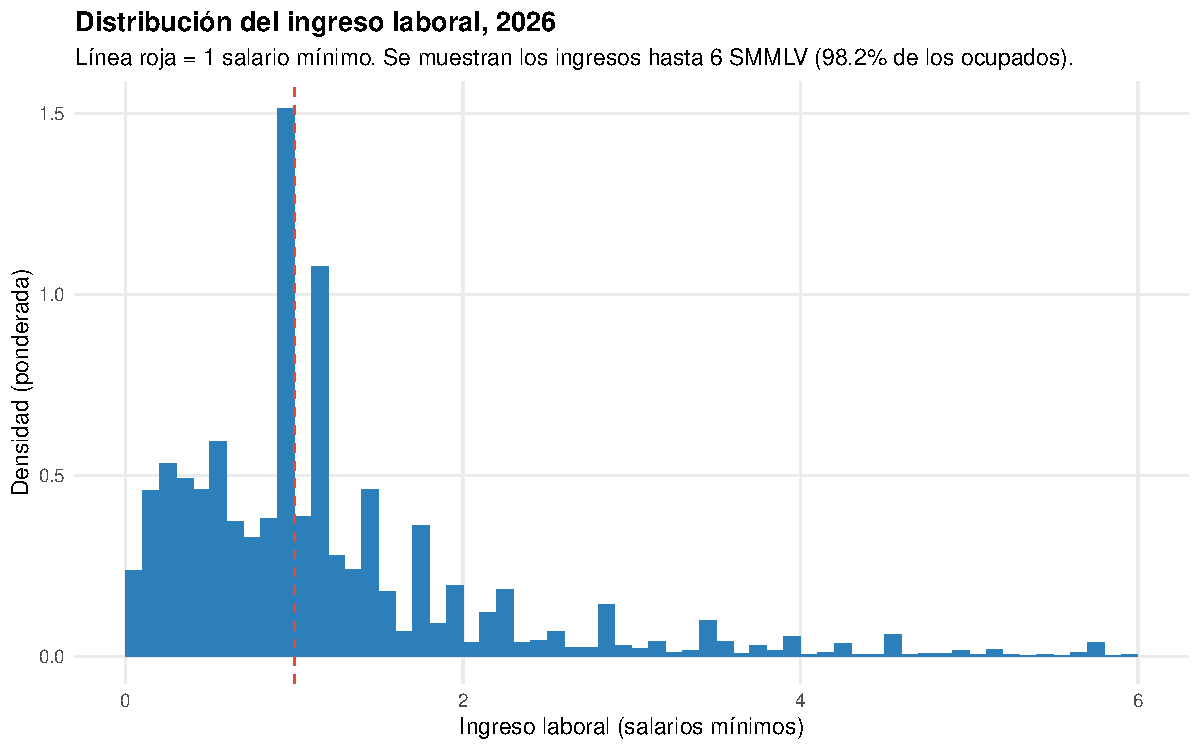
\includegraphics[width=0.85\textwidth]{07a_histograma_ingreso}
  \caption{Distribución del ingreso laboral, 2026 (ponderada)}
  \label{fig:histograma}
\end{figure}
% Interpretación: pico en el salario mínimo.

\begin{figure}[H]
  \centering
  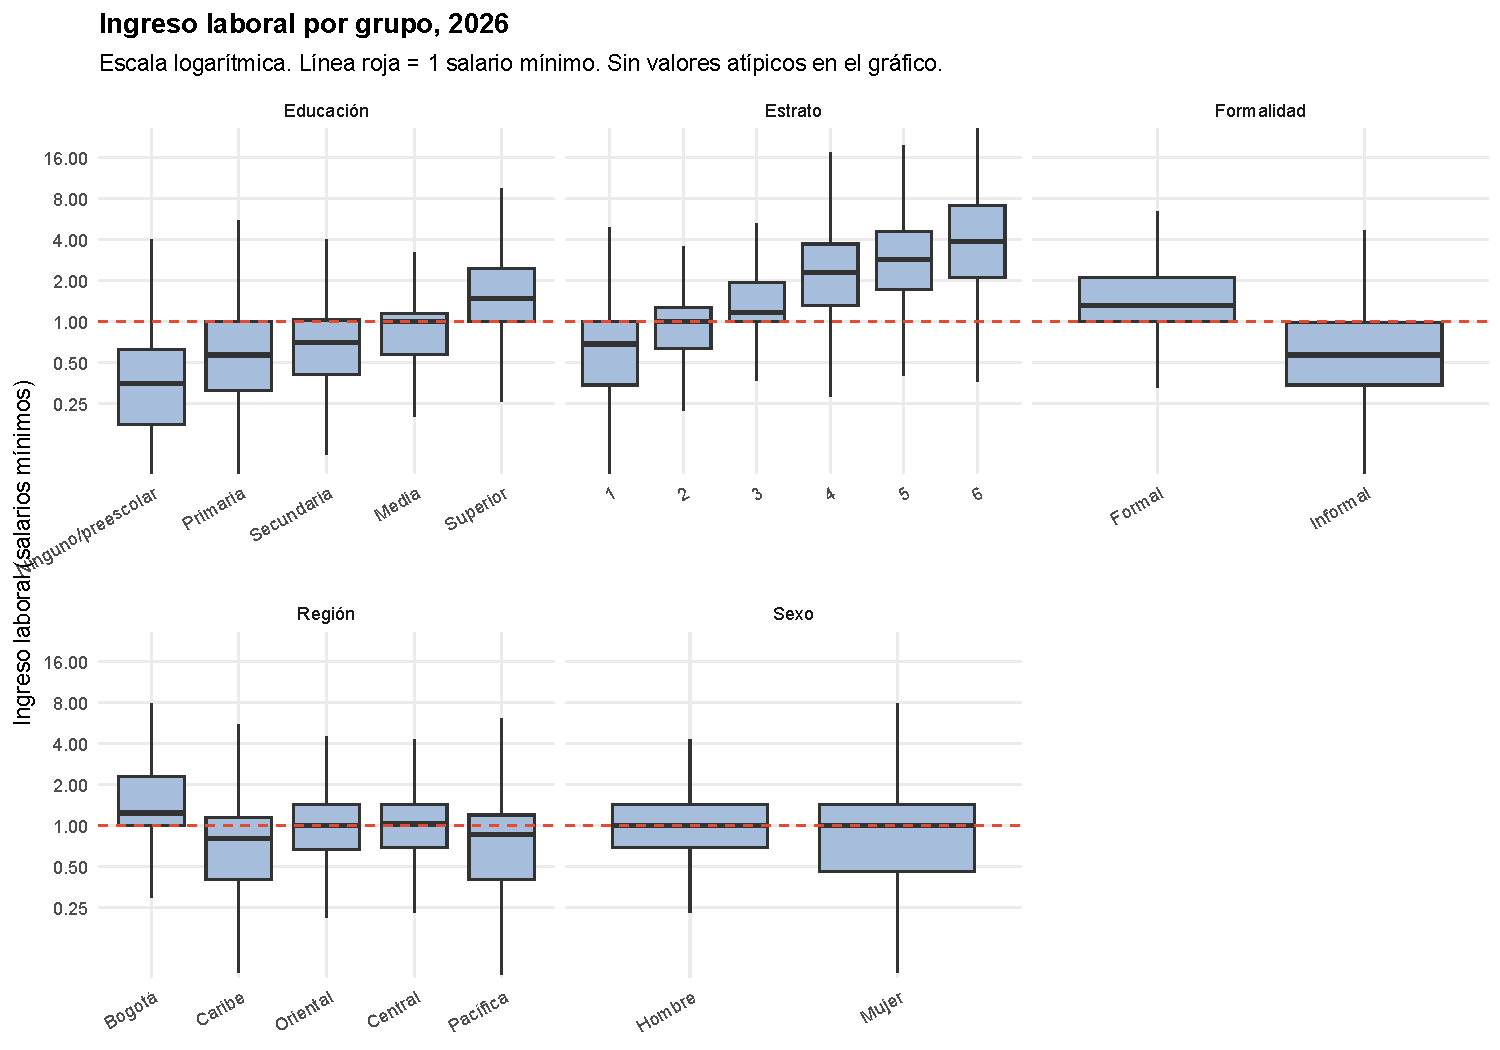
\includegraphics[width=\textwidth]{04_cajas_ingreso_por_grupo}
  \caption{Ingreso laboral por grupo, 2026}
  \label{fig:cajas}
\end{figure}
% Interpretación: diferencias entre grupos = intuición del componente "entre".

% Otras salidas disponibles (anexo o cuerpo, según el espacio):
%   tablas:  02_frecuencias_cuantitativas_agrupadas, 03_frecuencias_cualitativas,
%            04_cruzada_*, 04_ingreso_por_grupo, 05_correlaciones, 06_evolucion
%   figuras: 03_barras_cualitativas, 05_dispersion_horas_ingreso,
%            07b_ln_ingreso_vs_normal, 07c_muestra_vs_poblacion

% ============================================================
\section{Resultados de la simulación (H1)}
% ~2 páginas. Tabla de sesgo, varianza, ECM y ER por estimador y tamaño de
% muestra; figura de ECM frente a n; prueba t pareada de H1.
% PENDIENTE: el script de la simulación todavía no existe (decisión D5).

% ============================================================
\section{Desigualdad del ingreso laboral, 2018--2026 (H2 y H3)}
% ~1,5 páginas.

\begin{table}[H]
  \centering
  \caption{Índice de Theil por año según el factor de expansión}
  \label{tab:theil}
  \tabla{theil_por_anio}
\end{table}
% fex_aj = estimador A (principal); FEX = A sin ajuste por no respuesta;
% sin_pesos = estimador B. Comentar el salto 2021–2022 (cambio de marco).

\begin{table}[H]
  \centering
  \caption{Porcentaje de la desigualdad explicado por cada dimensión (componente entre)}
  \label{tab:entre}
  \tabla{theil_participacion_entre}
\end{table}
% H2: comparar educación con las demás dimensiones en 2026 (con IC bootstrap).
% H3: diferencia 2026 − 2018 con IC bootstrap y su sensibilidad a la limpieza
%     (docs/AUDITORIA.md, §2.8). Reportar el resultado aunque contradiga la hipótesis.
% PENDIENTE: el bootstrap todavía no existe.

% ============================================================
\section{Inferencia clásica}
% ~1 página. Resultados de P1–P7 y su interpretación; tamaños de efecto, no solo
% valores p.

\begin{table}[H]
  \centering
  \caption{Intervalos de confianza y pruebas de hipótesis (submuestra de 2.000, 2026)}
  \label{tab:pruebas}
  \tablaancha{resumen_pruebas}
\end{table}

\begin{figure}[H]
  \centering
  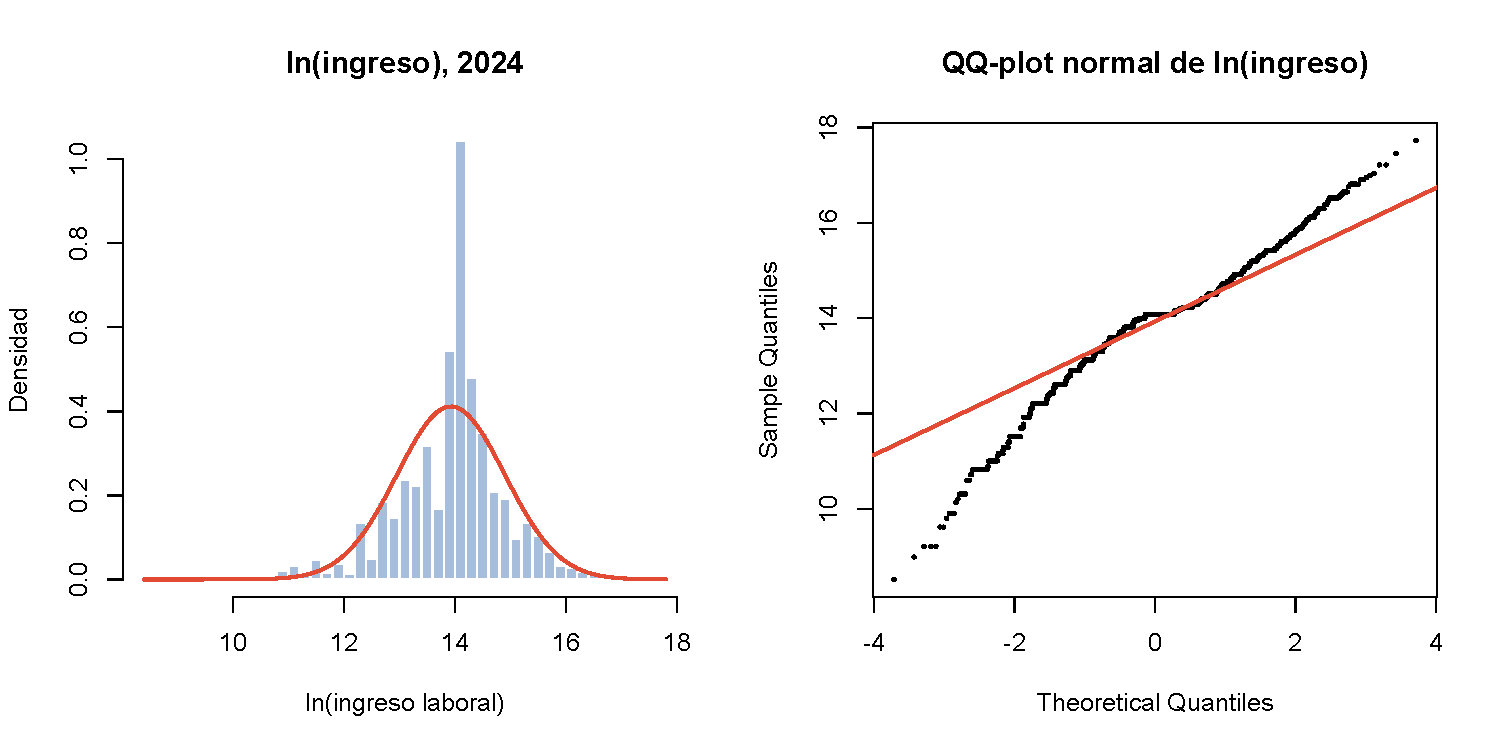
\includegraphics[width=\textwidth]{p7_ln_ingreso_normalidad}
  \caption{¿Es lognormal el ingreso? Histograma y QQ-plot de ln(ingreso), 2024}
  \label{fig:normalidad}
\end{figure}
% Otras salidas: p1_ic_media_ln_ingreso, p5_tabla_educ_formal,
% p6_regresion_coeficientes (tablas); p6_residuos (figura).

% ============================================================
\section{Discusión y limitaciones}
% ~0,5 páginas. Cambio de marco en 2022, no respuesta, estrato faltante,
% conglomerados ignorados, dimensiones correlacionadas (P5), asociación ≠ causalidad.

% ============================================================
\section{Conclusiones}
% ~0,5 páginas. Responder la pregunta; qué se concluye de H1, H2 y H3.

% ============================================================
\section*{Roles del equipo}
% La rúbrica evalúa los roles y responsabilidades de cada integrante.
% Tabla breve: integrante y qué hizo.

% ============================================================
\clearpage
\printbibliography[title={Referencias}]

% ============================================================
\clearpage
\appendix
\section{Anexos}
% Trazabilidad de la depuración (data/intermedia/etapa2_analitica/reportes/),
% libro de códigos (data/codebook.md), tablas completas de la descriptiva,
% descomposición por grupo de todos los años, detalle de las pruebas clásicas,
% sensibilidad a la no respuesta y al estrato faltante.

\end{document}
